\begin{pa} \label{PA:4.3}
Consider the applet found at \href{http://gvsu.edu/s/a9}{\texttt{http://gvsu.edu/s/aw}}\footnote{Marc Renault, Shippensburg University, Geogebra Applets for Calclulus, \href{http://gvsu.edu/s/5p}{\texttt{http://gvsu.edu/s/5p}}.}.  There, you will initially see the situation shown in Figure~\ref{F:4.3.GGBApplet}.
\begin{figure}[h]
\begin{center}
\scalebox{0.4}{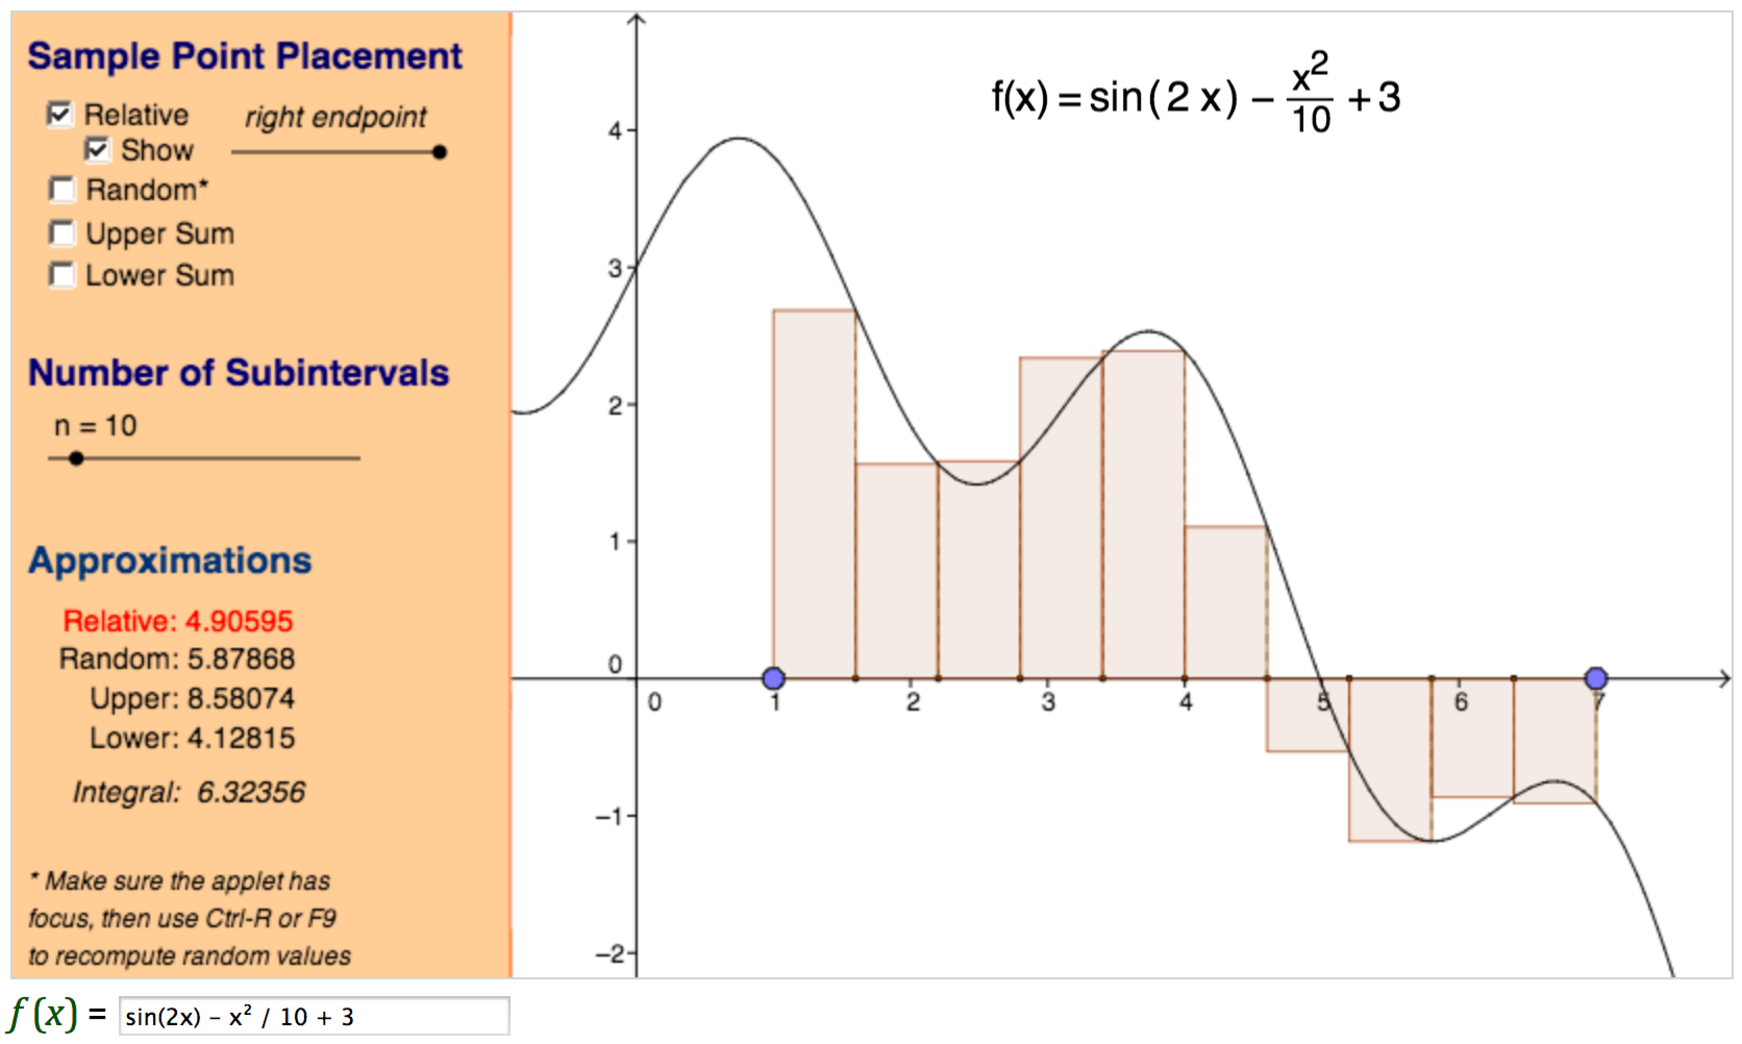
\includegraphics{figures/4_3_GGBApplet.pdf}}
\caption{A right Riemann sum with 10 subintervals for the function $f(x) = \sin(2x) - \frac{x^2}{10} + 3$ on the interval $[1,7]$.  The value of the sum is $R_{10} = 4.90595$.} \label{F:4.3.GGBApplet}
\end{center}
\end{figure}
Note that the value of the chosen Riemann sum is displayed next to the word ``relative,'' and that you can change the type of Riemann sum being computed by dragging the point on the slider bar below the phrase ``sample point placement.''

Explore to see how you can change the window in which the function is viewed, as well as the function itself.  You can set the minimum and maximum values of $x$ by clicking and dragging on the blue points that set the endpoints; you can change the function by typing a new formula in the ``f(x)'' window at the bottom; and you can adjust the overall window by ``panning and zooming'' by using the Shift key and the scrolling feature of your mouse.  More information on how to pan and zoom can be found at \href{http://gvsu.edu/s/Fl}{\texttt{http://gvsu.edu/s/Fl}}. 

Work accordingly to adjust the applet so that it uses a left Riemann sum with $n = 5$ subintervals for the function is $f(x) = 2x + 1$.  You should see the updated figure shown in Figure~\ref{F:4.3.GGBApplet2}.  Then, answer the following questions.
\begin{figure}[h]
\begin{center}
\scalebox{0.4}{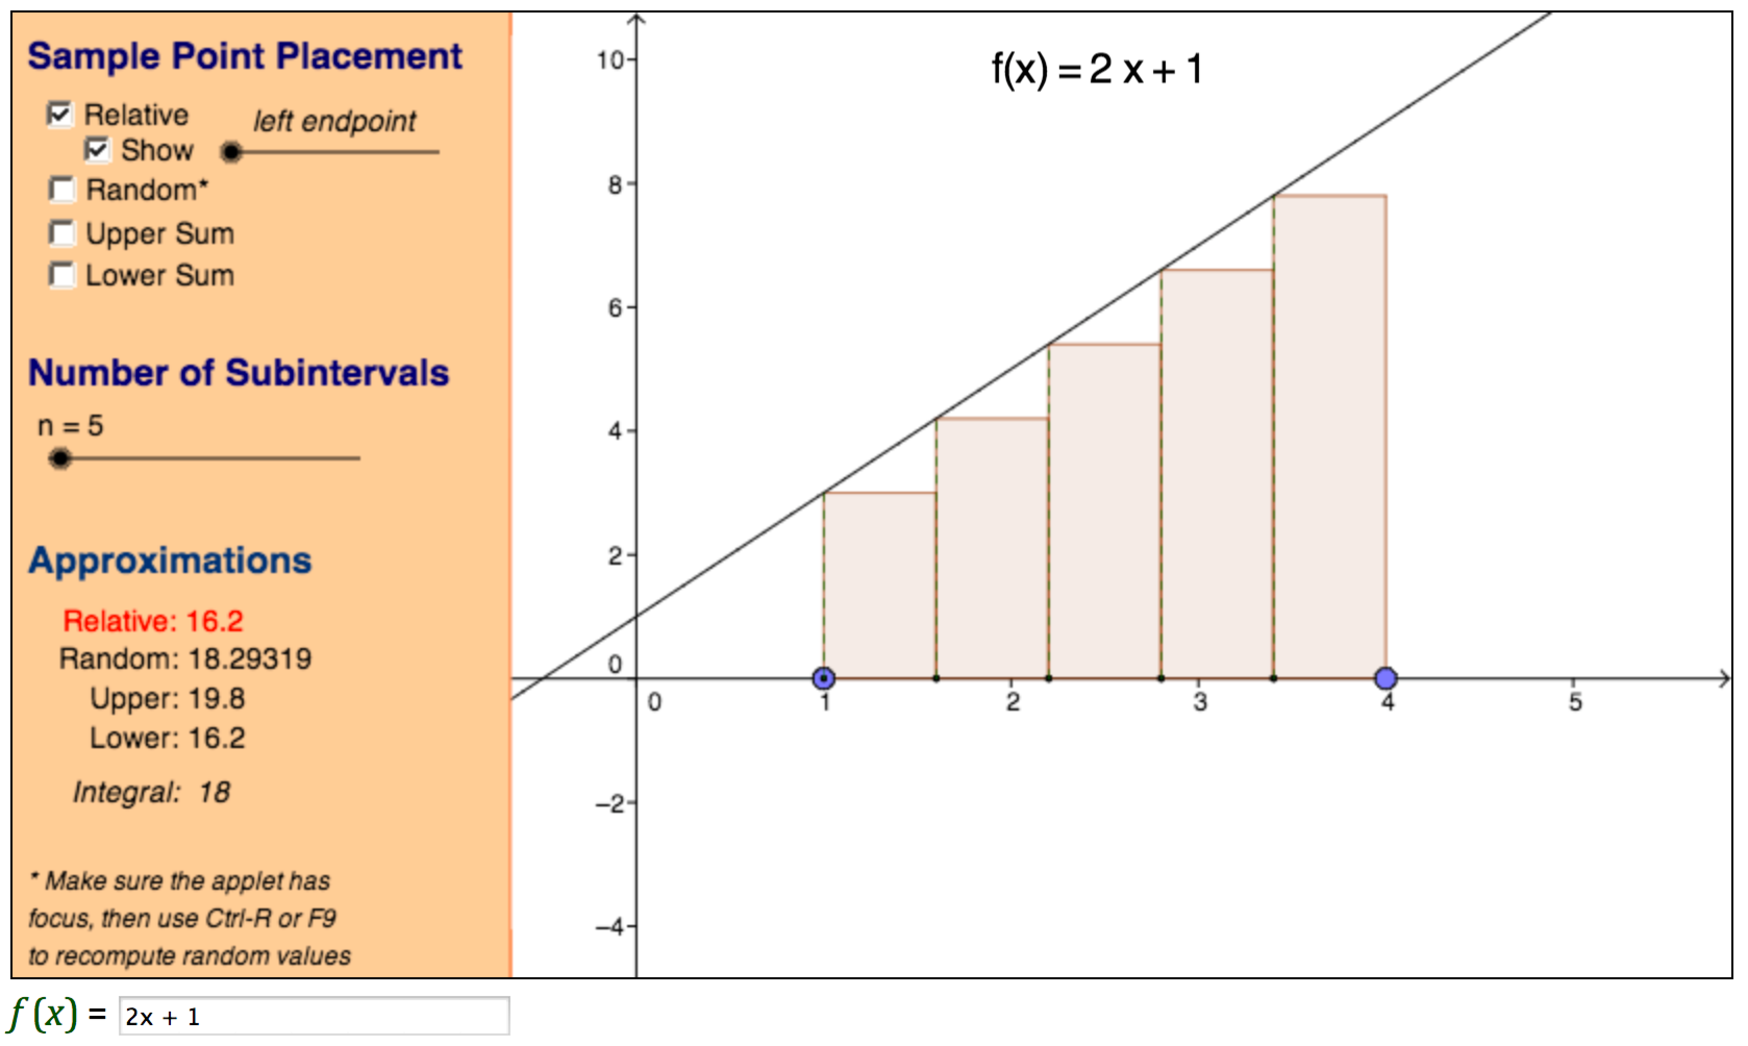
\includegraphics{figures/4_3_GGBApplet2.pdf}}
\caption{A left Riemann sum with 5 subintervals for the function $f(x) = 2x+1$ on the interval $[1,4]$.  The value of the sum is $L_5 = 16.2$.} \label{F:4.3.GGBApplet2}
\end{center}
\end{figure}
%Note that the value of the Riemann sum of our choice is displayed in the upper left corner of the window.  Further, by updating the value in the ``Intervals'' window and/or the ``Method'', we can see the different value of the Riemann sum that arises by clicking the ``Compute!'' button.
\ba
	\item Update the applet (and view window, as needed) so that the function being considered is $f(x) = 2x+1$ on $[1,4]$, as directed above.  For this function on this interval, compute $L_{n}$, $M_{n}$,  $R_{n}$ for $n = 5$, $n = 25$, and $n = 100$.  What appears to be the exact area bounded by $f(x) = 2x+1$ and the $x$-axis on $[1,4]$?
	\item Use basic geometry to determine the exact area bounded by $f(x) = 2x+1$ and the $x$-axis on $[1,4]$.
	\item Based on your work in (a) and (b), what do you observe occurs when we increase the number of subintervals used in the Riemann sum?
	\item Update the applet to consider the function $f(x) = x^2 + 1$ on the interval $[1,4]$ (note that you need to enter ``\texttt{x$\wedge$2 + 1}'' for the function formula).  Use the applet to compute $L_{n}$, $M_{n}$,  $R_{n}$ for $n = 5$, $n = 25$, and $n = 100$.  What do you conjecture is the exact area bounded by $f(x) = x^2+1$ and the $x$-axis on $[1,4]$?
	\item Why can we not compute the exact value of the area bounded by $f(x) = x^2+1$ and the $x$-axis on $[1,4]$ using a formula like we did in (b)?
\ea
\end{pa} 
\afterpa